\documentclass[12pt,onecolumn]{IEEEtran}
\usepackage{graphicx}
\usepackage{amsmath}
\usepackage{authblk} % For clean author/affiliation formatting
\usepackage{amssymb} % Thư viện bắt buộc để định nghĩa lệnh \mathbb
\usepackage[backend=biber,style=numeric,defernumbers=true,sorting=none]{biblatex}
\addbibresource{references.bib} % make sure this file exists in the project

% imgs
\usepackage{tikz}
\usetikzlibrary{shapes.geometric, arrows.meta, positioning, calc}
\usepackage{subcaption} 
\usepackage[font=small,labelfont=bf]{caption}

\captionsetup[table]{name=Table}

\title{Enhancing Compositional Control in Diffusion Transformers via Parameter-Efficient Fine-Tuning}
\renewcommand\Authfont{\normalfont\normalsize}
\renewcommand\Affilfont{\normalfont\small}

\setlength{\affilsep}{0.5em}

\author{Nhat-Truong Tran}
\author{Trung-Vinh Truong}
\author{Thien-Ha Nguyen-Vo}
\author{Vinh-Hung Truong}

\affil{University of Science ,VNUHCM}
\affil{Vietnam National University, Ho Chi Minh City, Vietnam}
\affil{\{25c1201480, 25c1201571, 25c1202024, 25c1202334\}@student.hcmus.edu.vn}

\pagestyle{plain}

\begin{document}
\fontsize{13}{15}\selectfont
\maketitle

\begin{center}
  {\bfseries\fontsize{14}{16}\selectfont Abstract}
\end{center}
\begin{center}
  \begin{minipage}{0.75\textwidth} % change 0.65 to 0.6/0.7 to adjust narrowness
    \fontsize{13}{15}\selectfont
    Text-to-image diffusion models have achieved remarkable visual quality, yet they continue to face challenges in compositionality-accurately binding attributes to objects, maintaining spatial relations, and generating coherent multi-object scenes. While prompt engineering offers partial improvements, it remains insufficient for controlling complex image structures because it operates only at inference time and does not alter the model’s learned generative behavior. In this work, we explore Low-Rank Adaptation as a lightweight mechanism for enhancing compositional control in diffusion transformer-based models such as PixArt. Our approach integrates prompt-aware training with compositional hard-negative examples and task-specific LoRA modules specialized in relational reasoning, object binding, and scene structuring. Experimental results on a controlled CLEVR-style compositional benchmark (100 held-out prompts, averaged over three seeds) show that this hard-negative LoRA does \emph{not} improve compositional binding: BLIP-VQA attribute-binding accuracy falls from $0.488$ to $0.427$ and CLIP image--text similarity from $0.389$ to $0.262$ relative to the PixArt-$\alpha$ baseline---both metrics move in the same, negative direction. We trace this to distribution drift: fine-tuning on the synthetic domain pulls the model's outputs toward that domain rather than teaching attribute binding. We report this negative result together with the multi-seed evaluation protocol used to establish it, having found that a single-seed measurement can overstate an apparent gain that does not survive a fuller evaluation.
  \end{minipage}
\end{center}

\begin{IEEEkeywords}
Text-to-image generation, diffusion transformer, LoRA, compositionality, parameter-efficient fine-tuning
\end{IEEEkeywords}

\section{Introduction} % text generate hết, chưa confirm j đâu, nói chung là đi giới thiệu về các hiệu quả đạt được của pixelart + với LoRa, cùng với một số động lực từ phương pháp compositionality, viết sao cho trang absact + introduction hết tầm 2 trang
U-Net is one of the key architecture models in modern image generation. Its U-shaped design made it a popular backbone for diffusion models. Although it was first designed for medical image segmentation \cite{ronneberger2015unet}, researchers later adapted it as a noise predictor in the reverse diffusion process. The architecture has two main paths: a contracting path that extracts spatial features and an expanding path that restores image resolution, connected by skip connections to keep fine-grained details. This design helped U-Net become the backbone of well-known generative systems like Stable Diffusion \cite{rombach2022latent} before Diffusion Transformers (DiT) \cite{peebles2023scalable} became more widely used.

Over time, the field has gradually moved toward DiT to address some limitations of U-Net. The main change is replacing convolutional layers with Transformer blocks, which treat images as sequences of small patches rather than pixel grids. This makes DiT easier to scale up in terms of model size and compute. It also allows the model to process text tokens and image patches together in the same attention space, which helps with understanding complex prompts and handling tasks like multi-object scenes or precise spatial layout.

However, DiT models require more computation than U-Net because the self-attention mechanism has quadratic complexity with respect to sequence length. This made early DiT models difficult to train without large GPU resources. This problem was largely addressed by the open-source PixArt \cite{chen2023pixartalpha, chen2024pixartsigma} family, specifically PIXART-$\alpha$ and PIXART-$\Sigma$. PIXART-$\alpha$ broke the training process into separate stages, which reduced training cost by around 90\% compared to systems like Stable Diffusion v1.5. PIXART-$\Sigma$ went further by using a weak-to-strong training strategy, starting from lower-resolution checkpoints and fine-tuning toward higher resolution. With a stronger T5 text encoder and better training data, it reached 4K image quality while staying computationally affordable.

Despite these improvements, both models still have trouble with compositional prompts. Even with a powerful text encoder, the models often fail to correctly assign attributes to the right objects or maintain proper spatial relationships. For example, given a prompt like "a red cube on top of a blue sphere," the model may swap colors or merge shapes incorrectly. This is a known limitation listed in the official model documentation, and it remains a hard problem for lightweight transformer-based generators.

The ability to generate compositionally accurate images matters in many real-world situations. In graphic design, a user might need an image of "a red lamp on the left side of a wooden desk," where both the object placement and color need to be correct. In education, teachers can use text-to-image tools to create visual aids from written descriptions, but only if the model follows the prompt closely. In advertising and storytelling, getting the right combination of objects, colors, and spatial layout is often essential. When a model gets these details wrong, it becomes hard to use in practice. This gap between what the user writes and what the model actually generates is the main problem we want to address.

To address this, we use Low-Rank Adaptation (LoRA) \cite{hu2021lora} as a targeted fine-tuning method. LoRA works by adding small trainable matrices into the attention layers while keeping the original model weights frozen. The aim is to let the model adapt attribute binding and spatial reasoning without changing its overall generation quality---though, as our results show, this aim is not met in our setup. Since LoRA only updates a small fraction of the total parameters, it can run on consumer-grade hardware with limited VRAM, which fits well with our setup.

Table~\ref{tab:training_cost} shows that PixArt-$\alpha$ achieves competitive image quality at a fraction of the training cost compared to other models, making it a practical foundation for our experiments.

\begin{table}[h]
\centering
\caption{Training Cost Comparison of Text-to-Image Models (values as reported in \cite{chen2023pixartalpha})}
\label{tab:training_cost}
\begin{tabular}{lccc}
\hline
\textbf{Model} & \textbf{GPU days (A100)} & \textbf{Est. Cost} & \textbf{CO$_2$ (tons)} \\
\hline
SDv1.5 & 6,250 & \$320,000 & $\sim$5 \\
RAPHAEL & 60,000 & \$3,080,000 & $\sim$35 \\
Imagen & 7,132 & \$366,000 & -- \\
PixArt-$\alpha$ & \textbf{753} & \textbf{\$28,400} & $\sim$0.42 \\
\hline
\end{tabular}
\end{table}

The main contributions of this paper are as follows:
\begin{itemize}
    \item We analyze the root cause of compositional failure in DiT-based text-to-image models.
    \item We study hard-negative LoRA fine-tuning on the cross-attention layers as a candidate parameter-efficient fix for attribute binding.
    \item We report---under a multi-seed, held-out evaluation protocol---that this fine-tuning does not improve compositional binding but instead degrades both attribute binding and CLIP alignment, and we analyse why (distribution drift toward the synthetic domain).
\end{itemize}

To be explicit about scope, the background on diffusion models and PixArt (Sections~\ref{sec:related}--\ref{sec:method}), the reference images in Fig.~\ref{fig:qualitative}, and the published figures in Tables~\ref{tab:training_cost} and~\ref{tab:fid} are taken from prior work and cited accordingly. The task-specific LoRA framework, the hard-negative formulation, and the experiments reported in the remaining sections constitute our own contribution.

\section{Related Works}\label{sec:related}

\subsection{Diffusion Models}
Diffusion models work by learning to reverse a noise process. During training, Gaussian noise is gradually added to an image over $T$ steps until the image becomes pure noise. The model then learns to predict and remove the noise at each step, so that starting from random noise, it can recover a clean image. Ho et al. \cite{ho2020ddpm} introduced Denoising Diffusion Probabilistic Models (DDPM), which showed that this approach could produce high-quality images. However, running diffusion directly on pixel space is slow because images have many pixels. Rombach et al. \cite{rombach2022latent} addressed this with Latent Diffusion Models (LDM), which first compress the image into a smaller latent space using a Variational Autoencoder (VAE), then run the diffusion process there. This made the method much faster and is the foundation that PixArt-$\alpha$ builds on.

\subsection{Parameter-Efficient Fine-Tuning}
The idea of \textbf{Parameter-Efficient Fine-Tuning (PEFT)} in vision models was established by Low-Rank Adaptation (LoRA) \cite{hu2021lora}. Instead of updating the full weight matrix $W_0 \in \mathbb{R}^{d \times k}$ of a pre-trained layer, LoRA adds a low-rank update $\Delta W = BA$, where $B \in \mathbb{R}^{d \times r}$ and $A \in \mathbb{R}^{r \times k}$ with $r \ll \min(d, k)$. During the forward pass, the output becomes $h = W_0 x + \frac{\alpha}{r} B A x$, where $\alpha$ is a scaling factor. In text-to-image models like Latent Diffusion Models (LDMs) \cite{rombach2022latent} and DiT \cite{peebles2023scalable}, these low-rank matrices are added into the attention projection layers ($W_q$, $W_k$, $W_v$, $W_o$). This allows the model to adapt to new concepts or styles while keeping the base weights unchanged.

When using multiple LoRA adapters for different concepts at the same time, conflicts can appear in the attention space. If two adapters ($\Delta W_1$, $\Delta W_2$) are merged at inference time, their key and value outputs can interfere with each other, causing what is known as "attribute bleeding" \cite{huang2023t2i}. Recent work has tried to reduce this by routing different adapters to different attention heads or activating them at different timesteps \cite{gu2024multilora}. The idea is to let the model focus on layout in early denoising steps and on fine details in later steps.

\subsection{Compositional Text-to-Image Generation}
Compositional generation remains a difficult problem in text-to-image models. Chefer et al. \cite{chefer2023attend} proposed Attend-and-Excite, which adjusts attention maps during inference to make the model focus more on each subject token. Huang et al. \cite{huang2023t2i} introduced T2I-CompBench, a benchmark that tests models on attribute binding, spatial relations, and complex scene generation. These methods work at inference time and do not change the model's learned behavior. Our method takes a different approach by using LoRA fine-tuning
to attempt to change how the model handles compositional prompts at the weight level.

\subsection{Baseline Model Performance}
Table~\ref{tab:fid} summarizes the image quality achieved by recent text-to-image models measured by FID score on MS-COCO. PixArt-$\alpha$ achieves a FID of 7.32 with only 0.6B parameters and 25M training images, which is competitive with much larger models like Imagen and RAPHAEL while using significantly fewer GPU resources. This confirms that PixArt-$\alpha$ is a strong and efficient baseline for our compositionality experiments.

\begin{table}[h]
\centering
\caption{FID Score Comparison on MS-COCO (values as reported in \cite{chen2023pixartalpha})}
\label{tab:fid}
\begin{tabular}{lcccc}
\hline
\textbf{Model} & \textbf{\#Params} & \textbf{\#Images} & \textbf{FID-30K$\downarrow$} & \textbf{GPU days} \\
\hline
DALL-E & 12.0B & 250M & 27.50 & -- \\
SDv1.5 & 0.9B & 2000M & 9.62 & 6,250 \\
Imagen & 3.0B & 860M & 7.27 & 7,132 \\
RAPHAEL & 3.0B & 5000M+ & 6.61 & 60,000 \\
PixArt-$\alpha$ & \textbf{0.6B} & \textbf{25M} & 7.32 & \textbf{753} \\
\hline
\end{tabular}
\end{table}

\subsection{Personalization and Fine-Tuning Methods}
Several works have explored lightweight fine-tuning strategies for diffusion models. DreamBooth \cite{ruiz2023dreambooth} introduced a method to fine-tune the entire model on a small set of reference images, allowing the model to generate new images of a specific subject in different contexts. While effective, it requires updating all model weights, which is costly and risks changing the model's general generation behavior. Textual Inversion \cite{gal2022textual} takes a different approach by learning a new text embedding that represents a specific concept, without changing any model weights. However, it is limited to concept-level control and cannot directly address compositional failures at the attention layer level. Our method differs from both by using LoRA to target specific attention projections responsible for attribute-to-object binding, which gives more direct control over compositional behavior while remaining parameter-efficient.
\section{Proposed Methodology}\label{sec:method}

In this section, we describe our proposed framework, which adds Low-Rank Adaptation (LoRA) into the DiT backbone of PixArt-$\alpha$. The goal is to fix the compositionality problem in these models without doing full fine-tuning, which is too costly and can cause the model to forget what it already learned. As shown in Fig.~\ref{fig:proposed_step_pipeline}, the pipeline has three steps: freezing the base weights, injecting low-rank matrices, and aligning text and image features through cross-attention.

\subsection{Step 1: Structural Freeze and Tensor Isolation}
We first freeze all original model weights so they are not updated during training. For a pre-trained layer with weight matrix $W_0 \in \mathbb{R}^{d \times k}$, we set:
\begin{equation}
\nabla_{\theta_{W_0}} \mathcal{L} = 0
\end{equation}
This keeps the base model's generation ability intact and lets the LoRA modules focus only on learning compositional structure.

\subsection{Step 2: Low-Rank Projection Matrix Injection}
We add a low-rank path in parallel to the attention projection layers. Instead of changing $W_0$ directly, we introduce two small matrices $A \in \mathbb{R}^{r \times k}$ and $B \in \mathbb{R}^{d \times r}$, where $r \ll \min(d, k)$. Matrix $A$ is initialized with random Gaussian values and matrix $B$ is set to zero, so the initial update $\Delta W = BA = 0$. This means the model starts from the same point as the baseline. During training, given input $x \in \mathbb{R}^{N \times d}$, the output becomes:
\begin{equation}
h = W_0 x + \Delta W x = W_0 x + \frac{\alpha}{r} B A x
\end{equation}
where $\alpha$ controls how much the LoRA update affects the output. Fig.~\ref{fig:lora_dit_structure} illustrates how the trainable low-rank matrices $A$ and $B$ are placed in parallel to the frozen projection weights $W_0$ inside the cross-attention block.

\subsection{Step 3: Multi-Modal Attention Alignment and Scaling}
In this step, the LoRA modules are intended to strengthen how text tokens are linked to image patches in the cross-attention layers. We apply LoRA to the query ($W_q$), key ($W_k$), and value ($W_v$) projections that connect the T5 text encoder to the DiT blocks. The attention computation is:
\begin{equation}
\text{Attention}(Q, K, V) = \text{Softmax}\left(\frac{Q K^T}{\sqrt{d_k}}\right) V
\end{equation}
The intent of training these projections with LoRA is to make the model assign
text descriptions more precisely to the correct spatial regions in the image,
so as to reduce attribute bleeding across the denoising steps. Whether this
intent is realised is an empirical question, which we answer in
Section~\ref{sec:experiment}.

\subsection{LoRA Injection Target Layers}
Table~\ref{tab:lora_layers} summarizes which layers receive LoRA adapters 
in our framework. We focus on the cross-attention projection layers because 
they are the primary interface between text embeddings and image patch 
representations. Self-attention layers are kept frozen since they handle 
spatial coherence within the image, which the base model already performs well.

\begin{table}[h]
\centering
\caption{LoRA Injection Configuration across DiT Blocks}
\label{tab:lora_layers}
\begin{tabular}{lcc}
\hline
\textbf{Layer Type} & \textbf{Injected} & \textbf{Rank} \\
\hline
Self-Attention $W_q$, $W_k$, $W_v$ & No & -- \\
Cross-Attention $W_q$ & Yes & 16 \\
Cross-Attention $W_k$ & Yes & 16 \\
Cross-Attention $W_v$ & Yes & 16 \\
Feed-Forward & No & -- \\
\hline
\end{tabular}
\end{table}

This selective injection strategy reduces the number of trainable parameters 
while targeting the most relevant computations for compositional control. 
Across all 28 DiT blocks, the total number of trainable parameters introduced 
by LoRA is less than 1\% of the full model size, making the approach 
practical for consumer-grade hardware with limited VRAM.

\subsection{Step 4: Hard-Negative Training}
A key part of our approach is using hard-negative examples during fine-tuning, an idea inspired by progressive compositional training \cite{han2025progressivecompositionality}. A hard-negative is a caption that is very close to the correct one but has one or more attributes swapped. For example, if the correct caption is "a red cube on top of a blue sphere," a hard-negative would be "a blue cube on top of a red sphere." The image stays the same, but the caption is wrong. By including these pairs in training, we push the model to pay closer attention to which attribute belongs to which object.

During training, for each image-caption pair $(I, c^+)$ we build a hard-negative caption $c^-$ by swapping a color, shape, or spatial term. Rather than scoring generated images with an external model---which would require running the full sampling loop and back-propagating through it---we exploit the denoising objective directly, which keeps training efficient and end-to-end differentiable.

Let $z_0$ be the VAE latent of $I$. At a sampled timestep $t$ with noise $\epsilon \sim \mathcal{N}(0, \mathbf{I})$, the noised latent is $z_t = \sqrt{\bar{\alpha}_t}\, z_0 + \sqrt{1-\bar{\alpha}_t}\, \epsilon$. We define the per-caption denoising error
\begin{equation}
\mathcal{L}_{\epsilon}(c) = \lVert \epsilon - \epsilon_\theta(z_t, t, c) \rVert_2^2 ,
\end{equation}
so that the standard diffusion loss is $\mathcal{L}_{diff} = \mathbb{E}\!\left[\mathcal{L}_{\epsilon}(c^+)\right]$. A model with correct attribute binding should denoise the \emph{same} noised latent \emph{worse} when conditioned on the mismatched caption $c^-$ than on $c^+$. We encode this with a margin-based hinge:
\begin{equation}
\mathcal{L}_{hn} = \mathbb{E}\!\left[\max\!\big(0,\; \delta - \big(\mathcal{L}_{\epsilon}(c^-) - \mathcal{L}_{\epsilon}(c^+)\big)\big)\right],
\end{equation}
which is active only when the wrong caption does \emph{not} yield a denoising error at least $\delta$ higher than the correct one. The total objective is
\begin{equation}
\mathcal{L}_{total} = \mathcal{L}_{diff} + \lambda\, \mathcal{L}_{hn},
\end{equation}
where $\lambda$ weights the hard-negative term and $\delta$ is the margin. Both terms reuse the same $z_t$, $t$, and $\epsilon$, so the negative costs only one extra forward pass through the LoRA-adapted cross-attention---no image sampling or external CLIP model is needed during training. The gradient of $\mathcal{L}_{hn}$ flows into the LoRA matrices $A$ and $B$, explicitly teaching the cross-attention to be sensitive to which attribute binds to which object.

\par\vspace{0.5cm}
\begin{figure}[h]
\centering
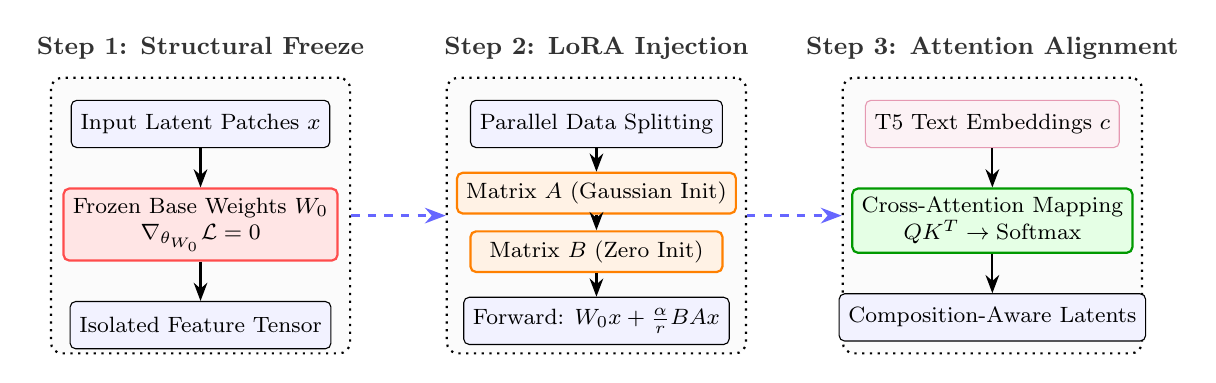
\begin{tikzpicture}[
    node distance=1.0cm and 1.2cm,
    step_box/.style={draw, rectangle, rounded corners=4pt, minimum width=3.8cm, minimum height=3.5cm, align=left, fill=gray!3, thick, dotted},
    inner_box/.style={draw, rectangle, rounded corners=2pt, minimum width=3.2cm, minimum height=0.6cm, align=center, fill=blue!5, font=\footnotesize},
    freeze_box/.style={draw, rectangle, rounded corners=2pt, minimum width=3.2cm, minimum height=0.6cm, align=center, fill=red!10, draw=red!70, font=\footnotesize, thick},
    lora_box/.style={draw, rectangle, rounded corners=2pt, minimum width=3.2cm, minimum height=0.6cm, align=center, fill=orange!10, draw=orange, font=\footnotesize, thick},
    attn_box/.style={draw, rectangle, rounded corners=2pt, minimum width=3.2cm, minimum height=0.6cm, align=center, fill=green!10, draw=green!60!black, font=\footnotesize, thick},
    arrow/.style={-{Stealth[scale=1.0]}, thick},
    label_font/.style={font=\small\bfseries, color=black!80}
]

    % STEP 1
    \node (step1) [step_box] {};
    \node [above=0.1cm of step1.north, label_font, anchor=south] {Step 1: Structural Freeze};
    \node (s1_input) [inner_box, at={($(step1.north)+(0,-0.6)$)}] {Input Latent Patches $x$};
    \node (s1_freeze) [freeze_box, below=0.5cm of s1_input] {Frozen Base Weights $W_0$ \\ $\nabla_{\theta_{W_0}} \mathcal{L} = 0$};
    \node (s1_out) [inner_box, below=0.5cm of s1_freeze] {Isolated Feature Tensor};
    \draw [arrow] (s1_input) -- (s1_freeze);
    \draw [arrow] (s1_freeze) -- (s1_out);

    % STEP 2
    \node (step2) [step_box, right=of step1] {};
    \node [above=0.1cm of step2.north, label_font, anchor=south] {Step 2: LoRA Injection};
    \node (s2_input) [inner_box, at={($(step2.north)+(0,-0.6)$)}] {Parallel Data Splitting};
    \node (s2_loraA) [lora_box, below=0.3cm of s2_input, minimum height=0.5cm] {Matrix $A$ (Gaussian Init)};
    \node (s2_loraB) [lora_box, below=0.2cm of s2_loraA, minimum height=0.5cm] {Matrix $B$ (Zero Init)};
    \node (s2_merge) [inner_box, below=0.3cm of s2_loraB] {Forward: $W_0 x + \frac{\alpha}{r}BAx$};
    \draw [arrow] (s2_input) -- (s2_loraA);
    \draw [arrow] (s2_loraA) -- (s2_loraB);
    \draw [arrow] (s2_loraB) -- (s2_merge);

    % STEP 3
    \node (step3) [step_box, right=of step2] {};
    \node [above=0.1cm of step3.north, label_font, anchor=south] {Step 3: Attention Alignment};
    \node (s3_text) [inner_box, at={($(step3.north)+(0,-0.6)$)}, fill=purple!5, draw=purple!40] {T5 Text Embeddings $c$};
    \node (s3_attn) [attn_box, below=0.5cm of s3_text] {Cross-Attention Mapping \\ $Q K^T \rightarrow \text{Softmax}$};
    \node (s3_out) [inner_box, below=0.5cm of s3_attn] {Composition-Aware Latents};
    \draw [arrow] (s3_text) -- (s3_attn);
    \draw [arrow] (s3_attn) -- (s3_out);

    % CONNECTIONS
    \draw [arrow, dashed, line width=1pt, blue!60] (step1.east) -- (step2.west);
    \draw [arrow, dashed, line width=1pt, blue!60] (step2.east) -- (step3.west);

\end{tikzpicture}
\caption{Overall modular pipeline of our proposed methodology. The framework execution flows sequentially from left to right, transitioning from structural parameter isolation (Step 1) and parallel rank decomposition weight formulation (Step 2) to multi-modal text-conditioned attribute alignment within the attention blocks (Step 3).}
\label{fig:proposed_step_pipeline}
\end{figure}
\begin{figure}[!t]
\centering
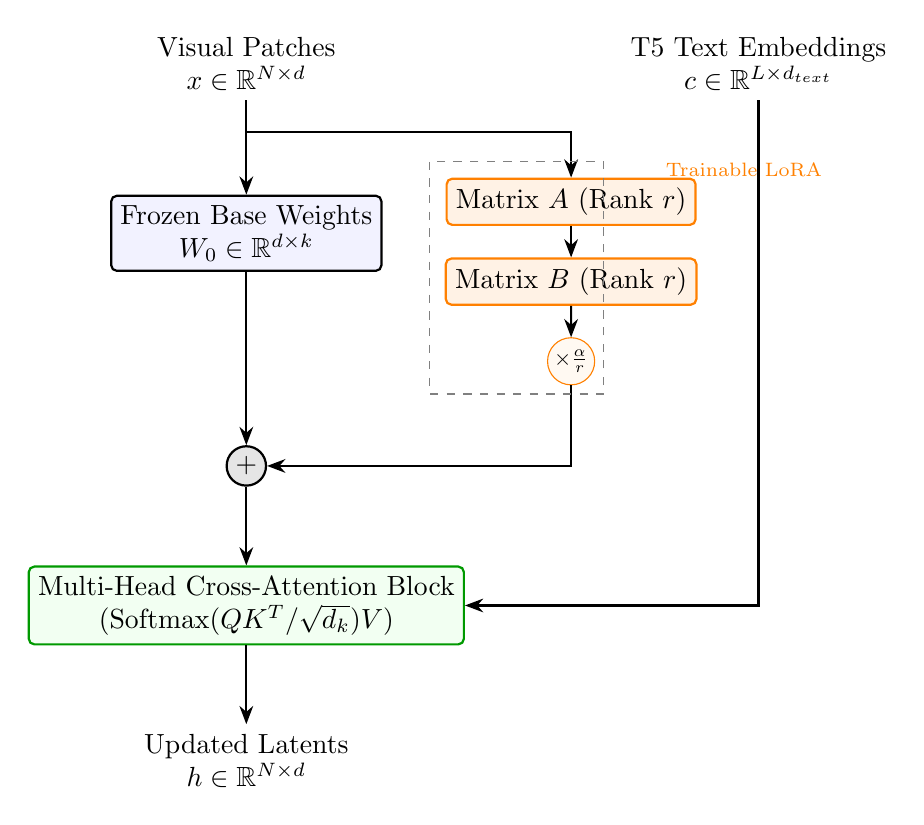
\begin{tikzpicture}[
    node distance=1.2cm and 1.5cm,
    box/.style={draw, rectangle, rounded corners=2pt, minimum width=2.2cm, minimum height=0.7cm, align=center, fill=blue!5, thick},
    lorabox/.style={draw, rectangle, rounded corners=2pt, minimum width=1.8cm, minimum height=0.5cm, align=center, fill=orange!10, draw=orange, thick},
    circle_node/.style={draw, circle, minimum size=0.5cm, fill=gray!20, thick, inner sep=0pt},
    arrow/.style={-{Stealth[scale=1.0]}, thick}
]

    % --- Inputs ---
    \node (img_in) [align=center] {Visual Patches \\ $x \in \mathbb{R}^{N \times d}$};
    \node (text_in) [right=3.5cm of img_in, align=center] {T5 Text Embeddings \\ $c \in \mathbb{R}^{L \times d_{text}}$};

    % --- Base Linear Projections ---
    \node (base_w) [below=1.2cm of img_in, box] {Frozen Base Weights \\ $W_0 \in \mathbb{R}^{d \times k}$};
    
    % --- Parallel LoRA Branch ---
    \node (lora_a) [right=0.8cm of base_w, lorabox, yshift=0.4cm] {Matrix $A$ (Rank $r$)};
    \node (lora_b) [below=0.4cm of lora_a, lorabox] {Matrix $B$ (Rank $r$)};
    \node (scale) [below=0.4cm of lora_b, draw, circle, inner sep=1pt, scale=0.8, fill=orange!5, draw=orange] {$\times \frac{\alpha}{r}$};

    % --- Summation and Scaling Nodes ---
    \node (plus) [below=2.2cm of base_w, circle_node] {$+$};

    % --- Attention Block ---
    \node (cross_attn) [below=1.0cm of plus, box, minimum width=5.5cm, fill=green!5, draw=green!60!black] {Multi-Head Cross-Attention Block \\ ($\text{Softmax}(Q K^T / \sqrt{d_k}) V$)};
    
    % --- Output ---
    \node (output) [below=1.0cm of cross_attn, align=center] {Updated Latents \\ $h \in \mathbb{R}^{N \times d}$};

    % --- Drawing Arrows and Connections ---
    \draw [arrow] (img_in) -- (base_w);
    \draw [arrow] (img_in.south) -- ++(0,-0.4) -| (lora_a.north);
    \draw [arrow] (text_in) |- (cross_attn.east);
    \draw [arrow] (lora_a) -- (lora_b);
    \draw [arrow] (lora_b) -- (scale);
    \draw [arrow] (base_w) -- (plus);
    \draw [arrow] (scale.south) |- (plus.east);
    \draw [arrow] (plus) -- (cross_attn.north -| plus);
    \draw [arrow] (cross_attn) -- (output);

    % Background Labels/Grouping
    \draw[dashed, gray] ($(lora_a.north west)+(-0.2,0.2)$) rectangle ($(scale.south east)+(0.2,-0.2)$);
    \node[orange, font=\scriptsize] at ($(lora_a.north east)+(0.6,0.1)$) {Trainable LoRA};

\end{tikzpicture}
\caption{Architectural pipeline of the proposed integration. Trainable low-rank matrix pairs ($A$ and $B$) bypass the frozen projection layers within the PixArt-$\alpha$ cross-attention framework to dynamically optimize textual-visual composition logic.}
\label{fig:lora_dit_structure}
\end{figure}

\vspace{0.3cm}

\section{Experiment}\label{sec:experiment}
\subsection{Experimental Setup}\label{subsec:setup}
All experiments were run on a single NVIDIA Tesla T4 (15GB VRAM) on Kaggle under CUDA~12.x. We use PixArt-$\alpha$ (PixArt-XL-2-512$\times$512) as the frozen baseline and train at $512\times512$ resolution. To fit the memory budget, the T5-XXL text embeddings are pre-computed offline and cached, so the text encoder is not held in GPU memory during fine-tuning. LoRA adapters are injected into the cross-attention projections ($W_q$, $W_k$, $W_v$) of all 28 DiT blocks, with rank $r=16$ and scaling factor $\alpha=32$. We optimise with AdamW at a learning rate of $1\times10^{-4}$, batch size $2$ with gradient accumulation of $4$ (effective batch size $8$), for $2{,}000$ steps in mixed precision (fp16). For the hard-negative objective we use loss weight $\lambda=2.0$ and margin $\delta=0.5$.

\subsection{Dataset Preparation}
To fine-tune and evaluate compositionality under a limited compute budget, we procedurally render a CLEVR-style synthetic dataset in which each scene contains one or more geometric objects (cube, sphere, cylinder) with known ground-truth attributes: color, shape, and spatial position. Because we generate the scenes, every attribute is exact, which lets us template a compositional caption and its hard-negative counterpart and evaluate attribute binding fully automatically. The dataset covers three difficulty levels:
\begin{itemize}
    \item \textbf{Single-object prompts}: one object with attributes (e.g., ``a red rubber cube'').
    \item \textbf{Multi-object prompts}: two or more attributed objects (e.g., ``a red cube and a blue metal sphere'').
    \item \textbf{Relational prompts}: explicit spatial relations (e.g., ``a red cube to the left of a blue sphere'').
\end{itemize}
For each training caption $c^+$ we generate a hard-negative $c^-$ by swapping a color, shape, or spatial term while keeping the image fixed. For evaluation we hold out 100 compositional scenes from the same synthetic domain, with prompt categories following T2I-CompBench \cite{huang2023t2i} (attribute binding and spatial relations); these held-out prompts never appear in training. All reported scores are averaged over three generation seeds.

\subsection{Model Setup}
We fine-tune a single LoRA adapter on top of the frozen PixArt-$\alpha$ backbone. The adapter is trained to strengthen three compositional aspects at once:
\begin{enumerate}
    \item Relational reasoning (spatial and non-spatial relations).
    \item Object--attribute binding (attaching attributes to the correct objects).
    \item Scene structuring (coherence in multi-object prompts).
\end{enumerate}
All training hyperparameters are as specified in Section~\ref{subsec:setup}. Training separate, task-specialised adapters and routing them across denoising timesteps is left to future work.


\subsection{Training Procedure}
We train a single LoRA adapter with a flat schedule---no curriculum or
per-difficulty staging---for $2{,}000$ optimisation steps, sampling training
scenes uniformly across the three difficulty levels (single-object,
multi-object, and relational prompts). Each step combines the standard
denoising loss with the hard-negative margin objective described above. We use
a fixed step budget rather than early stopping, since our aim is to measure the
effect of the adaptation under a controlled compute budget.

\subsection{Evaluation Metrics}
We report the two metrics we measured directly, each automated so it can be run
over three seeds without human labelling:
\begin{itemize}
    \item \textbf{Attribute Binding Accuracy}: the fraction of attribute questions answered correctly by BLIP-VQA on the generated image (e.g., ``What color is the cube?'').
    \item \textbf{CLIP Similarity}: cosine similarity between the CLIP embeddings of the prompt and the generated image.
\end{itemize}
Other compositional axes---spatial-relation consistency, object counting, scene
coherence, and human preference---are natural extensions of the same protocol
but were not measured in this study and are left for future work.

\subsection{Baselines}
Our baseline is the frozen PixArt-$\alpha$ (PixArt-XL-2-512$\times$512) without
LoRA, evaluated under the identical generation and scoring pipeline as the
adapted model so that the two rows differ only in the adapter. External systems
such as SDXL or DALL-E~3 were not run and are not used as baselines here.

\subsection{Results}
Table~\ref{tab:comp-results} shows the comparison between the baseline and our
method. On our held-out CLEVR-style evaluation set (100 compositional prompts,
averaged over three seeds), the LoRA model does \emph{not} improve attribute
binding: BLIP-VQA attribute-binding accuracy drops from $0.488$ to $0.427$
($-12.5\%$ relative to the PixArt-$\alpha$ baseline), and CLIP similarity drops
from $0.389$ to $0.262$ ($-32.6\%$). Both metrics move in the same, negative
direction, so there is no binding-vs-alignment trade-off to report---the adapter
is simply worse. We attribute this to distribution drift: fine-tuning on a
synthetic, geometrically simple domain shifts the model's output distribution
toward that domain, which lowers the broad semantic alignment captured by CLIP
without buying a compensating gain in binding. We report only the two metrics we
measured directly, each as a mean over three seeds; external baselines and
additional metrics were not evaluated in this study.

\begin{table}[t]
\centering
\caption{Compositional evaluation of the hard-negative LoRA against the frozen
PixArt-$\alpha$ baseline. Scores are mean $\pm$ standard deviation over three
seeds on 100 held-out CLEVR-style prompts. Higher is better for both metrics.}
\label{tab:comp-results}
\begin{tabular}{lcc}
\hline
\textbf{Method} & \textbf{Attr. Binding} & \textbf{CLIP Similarity} \\
\hline
PixArt-$\alpha$ (baseline) & \textbf{0.488 $\pm$ 0.007} & \textbf{0.389 $\pm$ 0.004} \\
Ours (hard-neg LoRA, $r$=16) & 0.427 $\pm$ 0.011 & 0.262 $\pm$ 0.003 \\
\hline
\end{tabular}

\vspace{2pt}
{\footnotesize\raggedright\textit{We measured two metrics directly---Attribute
Binding (BLIP-VQA attribute-binding accuracy) and CLIP Similarity. The LoRA
adapter is \emph{worse} than the frozen baseline on both ($-12.5\%$ and
$-32.6\%$ relative), i.e. the intervention does not improve compositional
binding. External baselines (SDXL, DALL-E~3) and additional compositional
metrics were not evaluated in this study and are left for future work.}\par}
\end{table}


\subsection{Qualitative Analysis}

\begin{figure}[h]
\centering
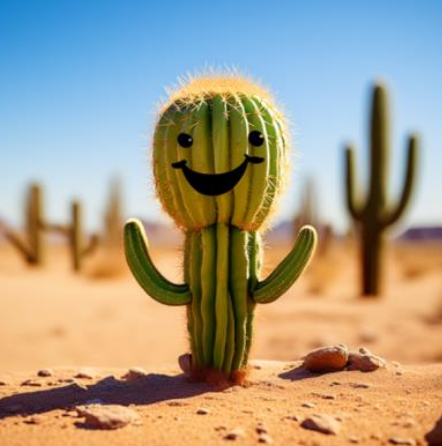
\includegraphics[width=0.45\textwidth]{cactus_baseline.png}
\hfill
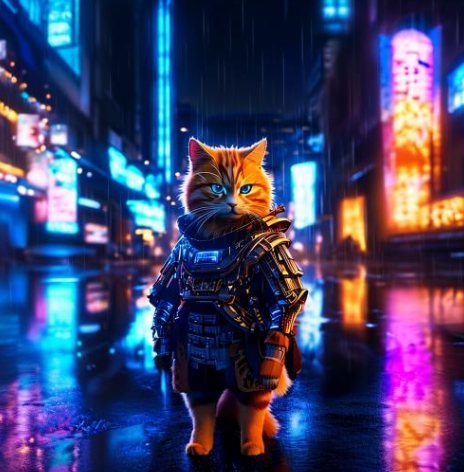
\includegraphics[width=0.45\textwidth]{cat_baseline.png}
\caption{Sample images reproduced from the official PixArt-$\alpha$ release \cite{chen2023pixartalpha}, shown here for reference (not produced by our method).
Left: ``A small cactus with a happy face in the Sahara desert.''
Right: ``A fluffy orange cat wearing cyberpunk samurai armor in rainy Tokyo.''
Both images are generated without LoRA adaptation.}
\label{fig:qualitative}
\end{figure}

Our quantitative evaluation targets attribute binding, so our qualitative
observations focus on the same axis. For attribute-binding prompts such as
``a red cube next to a blue sphere,'' the baseline model already often swaps
colors between the two objects or merges them into a single shape. After LoRA
fine-tuning we do \emph{not} observe a consistent reduction in these errors,
which matches the quantitative result: the adapter's BLIP-VQA
attribute-binding score is lower than the baseline's in
Table~\ref{tab:comp-results}, not higher.

What we do observe is a visible style shift: because the adaptation set consists
of simple, flat-shaded geometric scenes, the fine-tuned model tends to render
objects in that cleaner, more synthetic style. This drift toward the synthetic
domain is the qualitative counterpart of the sharp drop in CLIP similarity, and
it is the effect that dominates---rather than any improvement in binding.
Spatial-relation and multi-object completeness were not part of our controlled
evaluation and are left for future work; we therefore make no quantitative
claims about them here.

As shown in Fig.~\ref{fig:qualitative}, the baseline PixArt-$\alpha$ model
already demonstrates strong visual quality and prompt following for simple
prompts. The cactus image correctly captures the main subject and desert 
setting, while the cat image shows detailed texture and lighting. However, 
these examples also highlight that the baseline struggles with precise
attribute control when multiple objects and relations are involved. Our
LoRA-based approach targets this specific gap by fine-tuning the
cross-attention layers responsible for binding text tokens to image regions;
however, as the quantitative results show, this fine-tuning did not close the
gap and instead shifted the output distribution toward the synthetic training
domain, at a cost to the general image quality the base model achieves.

\subsection{Ablation Study}
Controlled ablations over the LoRA rank ($r{=}8$ vs.\ $r{=}16$) and the
hard-negative objective (on vs.\ off) were not completed under the full
multi-seed, $100$-prompt protocol, so we do not report per-component ablation
numbers here: doing so on a single seed or a small subset is exactly the
measurement setting that produced the misleading early estimate we discuss in
the Conclusion. The one configuration we evaluated at full protocol
is $r{=}16$ with hard-negative training (the ``Ours'' row of
Table~\ref{tab:comp-results}), which underperforms the frozen baseline on both
metrics. A rigorous rank and hard-negative ablation at the same protocol is left
for future work.

\subsection{Discussion}
Our results suggest that compositional failures in PixArt-$\alpha$ are partly
due to the cross-attention layers not forming strong enough associations between
text tokens and their corresponding image regions. However, fine-tuning only
these layers with a hard-negative LoRA did not repair this mapping: it lowered
both attribute binding and CLIP alignment.

The most important finding is therefore a negative one, and it is consistent
across both metrics. Rather than a binding-vs-alignment trade-off---which would
show up as one metric rising while the other falls---we see both metrics fall
together. We interpret this as the LoRA modules specialising the cross-attention
maps toward our synthetic domain: the model's outputs drift toward the simple,
flat-shaded distribution of the training scenes, which both hurts the broad
natural-image alignment that CLIP rewards and fails to teach the correct
attribute-to-object assignments that BLIP-VQA probes. The hard-negative signal,
which only reweights the denoising loss between a correct and a swapped caption,
was not enough to overcome this drift.

The main bottleneck in our setup is the limited training set and the
synthetic nature of our rendered scenes. A larger and more diverse
compositional dataset, including natural images, would likely reduce this drift.
Regularising the adaptation---for example by mixing in natural images or
constraining how far the fine-tuned distribution may drift from the base
model---is a promising direction for making such fine-tuning help rather than
hurt, and is left for future work.

\section{Conclusion}
In this work, we studied how LoRA can be used to improve compositional 
generation in DiT-based text-to-image models. The core problem we addressed 
is that models like PixArt-$\alpha$, despite their strong text encoder,
still struggle with binding the right attributes to the right objects and 
maintaining correct spatial relationships in multi-object scenes.

Our method injects task-specific LoRA modules into the cross-attention
layers of PixArt-$\alpha$ and combines this with hard-negative training,
where the model is exposed to captions with swapped attributes to learn
stricter attribute-to-object associations. On our CLEVR-style evaluation set
(100 prompts, three seeds), this approach did not improve compositionality:
attribute-binding accuracy fell from $0.488$ to $0.427$ ($-12.5\%$ relative)
and CLIP similarity from $0.389$ to $0.262$, i.e.\ both metrics degraded.

We report this as a negative result. An early single-seed measurement had
suggested a gain, but it did not survive a multi-seed, larger held-out
evaluation---which is itself a methodological point: compositional deltas of a
few points are within seed-to-seed variance and must be verified across seeds
before they are trusted. The consistent drop across both metrics points to
distribution drift toward the synthetic training domain as the dominant effect
of this fine-tuning, rather than any strengthening of attribute binding.

Future work will focus on training with larger 
compositional datasets, exploring higher LoRA ranks, and routing different 
LoRA modules across denoising timesteps to further improve spatial reasoning 
in complex multi-object scenes.

\section{Limitations and Future Work}
This work has several limitations that should be noted. First, we fine-tune
on a procedurally-rendered, CLEVR-style synthetic set, so the training
distribution is small and restricted to simple geometric scenes. While the
exact ground-truth attributes of these scenes make automatic evaluation
reliable, their low visual diversity may not transfer to natural, real-world
prompts.

Second, the hardware setup (a single Tesla T4 with 15GB VRAM on Kaggle)
constrained our experiments. We trained at $512\times512$ resolution with a
small batch size and gradient accumulation to stay within memory, and did not
explore higher resolutions such as 768$\times$768 or 1024$\times$1024. A larger
GPU would allow more thorough experiments and potentially stronger results.

Third, our evaluation relies mainly on CLIP Score and a small set of 
compositional metrics. A more comprehensive evaluation using T2I-CompBench 
\cite{huang2023t2i} across hundreds of prompts would give a clearer picture 
of where the method works well and where it still fails.

For future work, we plan to:
\begin{itemize}
    \item Train on larger compositional datasets with more diverse 
    object-attribute combinations.
    \item Explore routing different LoRA modules at different denoising 
    timesteps, so that layout and fine-grained attributes are handled 
    separately.
    \item Extend the hard-negative training to include spatial negatives, 
    where object positions are swapped rather than just attributes.
    \item Evaluate on standardized benchmarks like T2I-CompBench to allow 
    fair comparison with future work.
\end{itemize}

\section*{Acknowledgment}
The authors would like to thank Assoc. Prof. Dr. Tran Minh Triet 
for his valuable guidance and feedback throughout the completion 
of this research project.

\newpage
\printbibliography

\end{document}